
\documentclass[a4paper,12pt]{scrbook}
\usepackage{amsmath,amssymb,amsthm}
\usepackage{fancyvrb}
\usepackage{parskip}
\usepackage{lastpage}
\usepackage{verbatim,boxedminipage,enumitem}
\usepackage{ifthen}
\usepackage{color,graphicx}
\usepackage{pgf}
\usepackage{longtable}
\usepackage{upquote}
%\usepackage[all]{xy}
\usepackage{tobiShell}
\usepackage{tikz}
\usetikzlibrary{automata}
\usetikzlibrary{arrows}
\usepackage{pgf,pgfarrows,pgfnodes}
\usepackage{pgfplots}
\usepackage{circuitikz}
\usetikzlibrary{circuits}
\usetikzlibrary{circuits.logic.US}
\usepackage{mymath}
\usepackage{python}
%------------------------------------------------------------------
% Verbatim for console window - single line frame, no line numbers
%------------------------------------------------------------------
\DefineVerbatimEnvironment%
 {console}{Verbatim}
 {frame=single}

%--------------------------------------------------------
% Remove the vertical spacing before and after Verbatim.
%--------------------------------------------------------
\usepackage{atbeginend}
\BeforeBegin{console}{\mbox{}\\ \begin{minipage}{\textwidth}\vspace{3pt}}
\AfterEnd{console}{\vspace{4pt} \end{minipage} \\ }

\begin{document}
\thispagestyle{empty}

\begin{center}
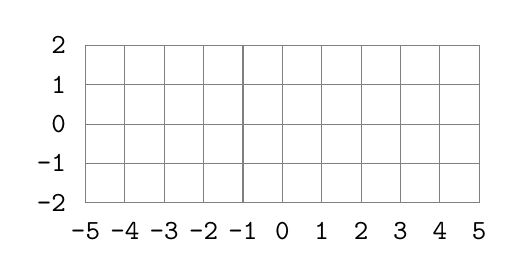
\begin{tikzpicture}[scale=0.5]
\draw[gray] (-5,-2) -- (-5,2);
\draw[gray] (-4,-2) -- (-4,2);
\draw[gray] (-3,-2) -- (-3,2);
\draw[gray] (-2,-2) -- (-2,2);
\draw[gray] (-1,-2) -- (-1,2);
\draw[gray] (0,-2) -- (0,2);
\draw[gray] (1,-2) -- (1,2);
\draw[gray] (2,-2) -- (2,2);
\draw[gray] (3,-2) -- (3,2);
\draw[gray] (4,-2) -- (4,2);
\draw[gray] (5,-2) -- (5,2);
\draw[gray] (-5,-2) -- (5,-2);
\draw[gray] (-5,-1) -- (5,-1);
\draw[gray] (-5,0) -- (5,0);
\draw[gray] (-5,1) -- (5,1);
\draw[gray] (-5,2) -- (5,2);
\draw(-5, -2) node [font=\ttfamily, label=below:{\texttt{-5}}] {};
\draw(-4, -2) node [font=\ttfamily, label=below:{\texttt{-4}}] {};
\draw(-3, -2) node [font=\ttfamily, label=below:{\texttt{-3}}] {};
\draw(-2, -2) node [font=\ttfamily, label=below:{\texttt{-2}}] {};
\draw(-1, -2) node [font=\ttfamily, label=below:{\texttt{-1}}] {};
\draw(0, -2) node [font=\ttfamily, label=below:{\texttt{0}}] {};
\draw(1, -2) node [font=\ttfamily, label=below:{\texttt{1}}] {};
\draw(2, -2) node [font=\ttfamily, label=below:{\texttt{2}}] {};
\draw(3, -2) node [font=\ttfamily, label=below:{\texttt{3}}] {};
\draw(4, -2) node [font=\ttfamily, label=below:{\texttt{4}}] {};
\draw(5, -2) node [font=\ttfamily, label=below:{\texttt{5}}] {};
\draw(-5, -2) node [font=\ttfamily, label=left:{\texttt{-2}}] {};
\draw(-5, -1) node [font=\ttfamily, label=left:{\texttt{-1}}] {};
\draw(-5, 0) node [font=\ttfamily, label=left:{\texttt{0}}] {};
\draw(-5, 1) node [font=\ttfamily, label=left:{\texttt{1}}] {};
\draw(-5, 2) node [font=\ttfamily, label=left:{\texttt{2}}] {};
\end{tikzpicture}

\end{center}

\end{document}
